\documentclass{article}
\usepackage{tikz}
\usepackage{amsmath}

\begin{document}

\[
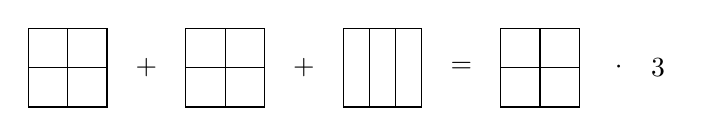
\begin{tikzpicture}
    % First term
    \draw (0, 0) rectangle (1, 1); % Outer box
    \draw (0.5, 0) -- (0.5, 1); % Vertical middle
    \draw (0, 0.5) -- (1, 0.5); % Horizontal middle
    \node at (0.25, 0.75) {\(\square\)}; % Add square inside

    \node at (1.5, 0.5) {\(+\)}; % Plus sign

    % Second term
    \draw (2, 0) rectangle (3, 1); % Outer box
    \draw (2.5, 0) -- (2.5, 1); % Vertical middle
    \draw (2, 0.5) -- (3, 0.5); % Horizontal middle
    \node at (2.25, 0.25) {\(\square\)}; % Square 1
    \node at (2.25, 0.75) {\(\square\)}; % Square 2

    \node at (3.5, 0.5) {\(+\)}; % Plus sign

    % Third term
    \draw (4, 0) rectangle (5, 1); % Outer box
    \draw (4.33, 0) -- (4.33, 1); % Divide into thirds
    \draw (4.66, 0) -- (4.66, 1); % Divide into thirds
    \node at (4.16, 0.5) {\(\square\)}; % Square 1
    \node at (4.5, 0.5) {\(\square\)}; % Square 2
    \node at (4.83, 0.5) {\(\square\)}; % Square 3

    \node at (5.5, 0.5) {\(=\)}; % Equals sign

    % Result (3 x term)
    \draw (6, 0) rectangle (7, 1); % Outer box
    \draw (6.5, 0) -- (6.5, 1); % Vertical middle
    \draw (6, 0.5) -- (7, 0.5); % Horizontal middle
    \node at (6.25, 0.25) {\(\square\)}; % Square 1
    \node at (6.25, 0.75) {\(\square\)}; % Square 2

    \node at (7.5, 0.5) {\(\cdot\)}; % Multiplication dot

    \node at (8, 0.5) {\(3\)}; % Coefficient
\end{tikzpicture}
\]
\end{document}
